%\documentclass{book}\usepackage{sjtfonts}\usepackage{includegraphics}\usepackage{alltt}\usepackage{latexsym}
%\begin{document}\input{defs0}%		miradefs.tex 		    June 1994

% opening and closing a quoted Miranda section

\newcommand{\mira}{\noindent\hrulefill\nopagebreak\so}
\newcommand{\arim}{\nopagebreak\st\hrulefill\\}

% backslash in the Miranda environment
% Only feasible approach is to use \verb+\+
% in line!

%\newcommand{\bs}{$\mi\backslash\!\!$}
%\newcommand{\lbs}{\mbox{\verb+\+}}

% ignoring part of the input

\newcommand{\ignore}[1]{}

% a blank line in a Miranda section

\newcommand{\bl}{\mbox{\ }}

% Signalling a diffculty.

\definecolor{light-gray}{gray}{0.95}

\newcommand{\beware}[2]
 {\medskip\noindent\colorbox{light-gray}{\parbox{\textwidth}
 {\mbox{\large\textbf{#1}} \medskip\noindent\\ #2}\medskip\noindent}}

% Subscripting in Miranda text
\newcommand{\subscr}[2]{\mbox{${\mbox{\texttt{#1}}}_{\mbox{\texttt{#2}}}$}}

%\newcommand{\subscr}[2]{\mbox{${\mbox{\mi #1}}_{\mbox{\smtt #2}}$}}
\newcommand{\aone}{\subscr{a}{1}}
\newcommand{\atwo}{\subscr{a}{2}}
\newcommand{\ak}{\subscr{a}{k}}

\newcommand{\aoneone}{\subscr{a}{1,1}}

\newcommand{\eone}{\subscr{e}{1}}
\newcommand{\etwo}{\subscr{e}{2}}
\newcommand{\ei}{\subscr{e}{i}}
\newcommand{\er}{\subscr{e}{r}}

\newcommand{\fone}{\subscr{f}{1}}
\newcommand{\fl}{\subscr{f}{l}}

\newcommand{\gone}{\subscr{g}{1}}
\newcommand{\gtwo}{\subscr{g}{2}}
\newcommand{\gi}{\subscr{g}{i}}
\newcommand{\gr}{\subscr{g}{r}}

\newcommand{\hone}{\subscr{h}{1}}
\newcommand{\hl}{\subscr{h}{l}}

\newcommand{\pone}{\subscr{p}{1}}
\newcommand{\ptwo}{\subscr{p}{2}}
\newcommand{\pk}{\subscr{p}{k}}

\newcommand{\qone}{\subscr{q}{1}}
\newcommand{\qtwo}{\subscr{q}{2}}
\newcommand{\qk}{\subscr{q}{k}}

\newcommand{\rone}{\subscr{r}{1}}
\newcommand{\rtwo}{\subscr{r}{2}}

\newcommand{\tone}{\subscr{t}{1}}
\newcommand{\ttwo}{\subscr{t}{2}}
\newcommand{\tn}{\subscr{t}{n}}

\newcommand{\vone}{\subscr{v}{1}}
\newcommand{\vtwo}{\subscr{v}{2}}
\newcommand{\vn}{\subscr{v}{n}}

% for regular expressions

\newcommand{\stone}{\subscr{st}{1}}
\newcommand{\sttwo}{\subscr{st}{2}}
\newcommand{\stn}{\subscr{st}{n}}
\newcommand{\rthree}{\subscr{r}{3}}

\newcommand{\eps}{$\varepsilon$}
\newcommand{\trans}[1]{\stackrel{\mbox{\tt #1}}{\longrightarrow}}



% superscript in Miranda text

\newcommand{\superscr}[2]{\mbox{${\mbox{\mi #1}}^{\mbox{\smtt #2}}$}}

% Not equals in Miranda text

\newcommand{\noteq}{\makebox[0pt][l]{=}/}
\newcommand{\overslash}{\makebox[0pt][l]{/}}

% Definitions in complexity chapter

\newfont{\oldSym}{cmsy10}
\newcommand{\Th}{\boldmath$\oldSym\Theta$}
\newcommand{\pow}[1]{\^{}#1}
\newcommand{\leqq}{$\leq$}
\newcommand{\geqq}{$\geq$}
\newcommand{\lll}{$\ll$}
\newcommand{\eqq}{$\equiv$}
\newcommand{\ltwo}{\subscr{log}{2}}

% Indexing

\newcommand{\minx}[1]{\index{#1@{\ttfamily{}#1}}}



\chapter{Getting started with Haskell programming}
\label{getStart}
\chapstart

\medskip
Chapter \ref{intro} introduced the foundations of functional programming in Haskell.
We are now ready to use GHCi to do some practical programming, and we introduce it here.

In beginning to program we will also learn the basics of the Haskell module 
system, under which programs can be written in multiple, interdependent files, 
and which can use the `built-in' functions in the prelude and libraries. 
Our programming
examples will concentrate on using the \texttt{Picture} example
introduced in Chapter \ref{intro} as well as some simple numerical
examples. 

In support of this we will look at how to get hold of the programs and
other background materials for the book from Hackage using Cabal, as well as how to obtain and install GHCi using GHCup. We will explore how to develop single-module programs using \texttt{ghci} as well as using \texttt{cabal repl} for more complex, multiple module projects.

We conclude by briefly surveying the kinds of error message that can
result from typing something incorrect into GHCi. 

\begin{figure}[t]
\begin{alltt}\minx{FirstScript.hs}
\input{FirstScript.hs}
\end{alltt}
\vspace*{-12pt}
\caption{An example script, \texttt{FirstScript.hs}.}
\label{FirstScript}
\end{figure}

\section[A first Haskell program]{A first Haskell program}
\markright{A first Haskell program}
 
We begin the chapter by giving a first Haskell program or
\textbf{script}\index{script}, which consists of the numerical examples from
Chapter \ref{intro}. This is the file
\texttt{FirstScript.hs}, shown in Figure \ref{FirstScript}. Haskell scripts are stored in files with the \textbf{extension}\index{extension}
`\texttt{.hs}'.\index{hs@\texttt{.hs}}





As well as definitions, a script will contain comments. 
A \textbf{comment}\index{comment} in a script
is a piece of information of value to a human reader rather than to a computer.
It might contain an informal explanation of how a function works,
how it should or should not be used, the overall design philosophy of a library and so on.
Everything in a program file is interpreted as
program text, \emph{except} where it is explicitly indicated that it is a
comment. 

Comments are indicated in two ways. The symbol
`\texttt{-{}-}'\minx{--} begins a comment\index{comment!symbol} which occupies the part of the
line to the right of the symbol. Comments can also be enclosed by the 
symbols `\texttt{\{-}'\minx{\{-} and `\texttt{-\}}'\minx{-\}}. These comments can be of
arbitrary length, spanning more than one line, as well as enclosing other comments; 
they are therefore
called \textbf{nested comments}\index{comment!nested}.

\section{Using Haskell in practice}
\index{GHCi|(}

The Glasgow Haskell Compiler (GHC)\index{Glasgow Haskell Compiler|see{GHC}}\index{GHC} is an industrial-strength compiler for Haskell. \textbf{GHC interactive (GHCi)} is an interactive interpreter based on GHC, which provides programmers with a Haskell \textbf{repl}, which successively \emph{reads} an expression, \emph{evaluates} it, \emph{prints} the result, and finally \emph{loops} back to the start. This is a great way to start programming, as it allows you to try out your ideas and experiment with definitions in the process of developing a program.

If you're learning Haskell in high school or college, or at work, your teachers or colleagues will have made sure it is available on the computers you use. If you want to install it for yourself on a machine that you control, the best, and easiest, way of working doing that is to use GHCup, \url{https://www.haskell.org/ghcup/}.

\begin{figure}[t] 
\begin{center}
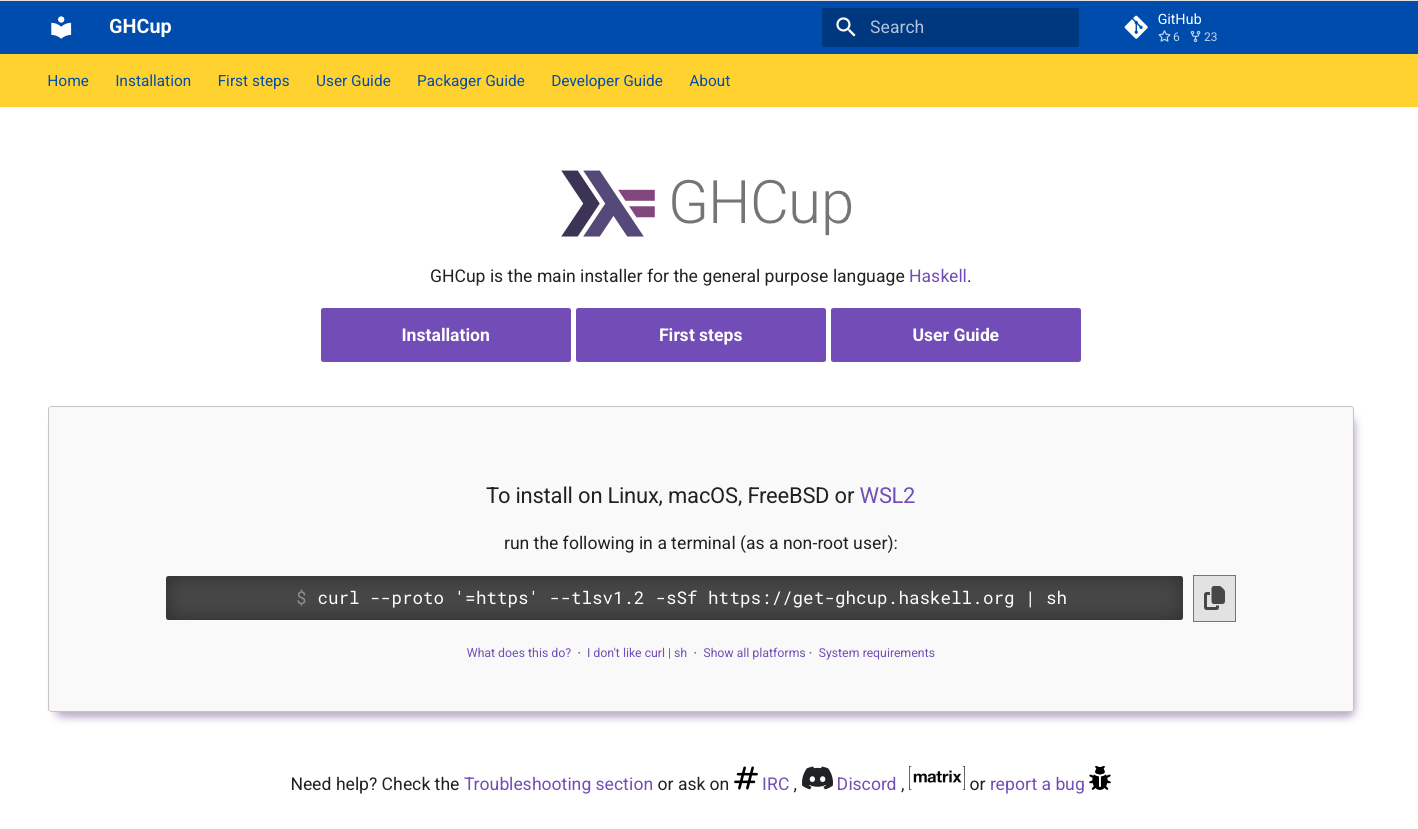
\includegraphics[width=\textwidth]{Pictures/GHCup.png}
\end{center} 
\caption{The GHCup homepage}
\label{GHCup}
\end{figure}

GHCup\index{GHCup} will install GHC, as well as some other components including \texttt{cabal},\index{Cabal} which is a package for distributing Haskell code and libraries, and one of the ways that you can access the code for the book;\index{downloading support materials}. If asked to select what to download, include \texttt{cabal}, and if you want to use Haskell within an IDE like VS Code, include the Haskell Language Server (HLS)\index{Haskell Language Server}\index{HLS} too. Also, you should follow the GHCup default of installing the \emph{recommended} versions of these programs.

Why should you consider using HLS? Development today is usually inside an Integrated Development Environment, or IDE, such as Visual Studio Code (VS Code). IDEs combines
editing with processing and running programs, as well as interacting with reposito-
ries, such as github, refactoring and other kinds of software tooling. To use Haskell most effectively within an IDE you will need to use the Haskell Language Server (HLS), which provides a rich enhancement of the editing functions of the IDE including type checking, refactoring,  integration with repositories and other support for software development.

We will come back to \texttt{cabal} and HLS when we discuss multi-file projects in Section \ref{multipleModuleProgs} and again when we discuss how to find out more about the functions and libraries in Haskell in Chapter \ref{progLists}.



 
Other ways of using Haskell -- such as using it online or in a browser -- can be found in Appendix \ref{OtherHS}.


\begin{figure}[t] 
\begin{center}
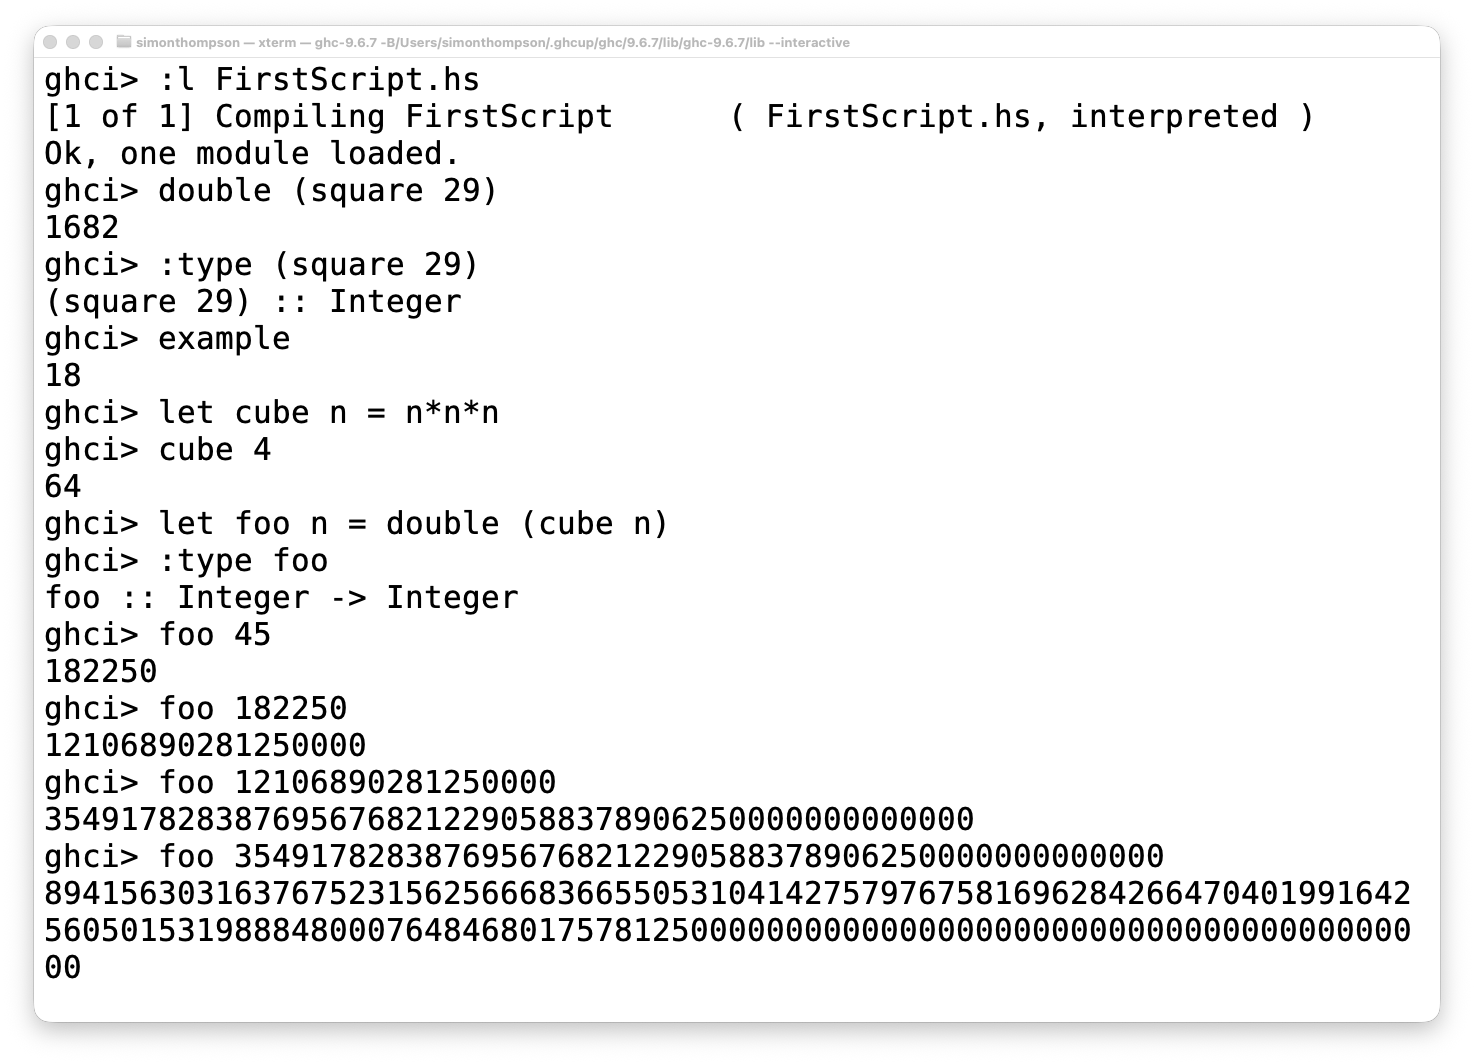
\includegraphics[width=\textwidth]{Pictures/ghci-terminal.png}
\end{center} 
\caption{A GHCi terminal session}
\label{GHCiSession}
\end{figure}


\section{Using GHCi}


In this text we describe the terminal-style interface to GHCi, illustrated in Figure
\ref{GHCiSession},
because this is common to macOS, Linux and Windows WSL. 

\subsection*{GHCi documentation}
\index{GHCi!documentation}

The GHCup webpage has documentation about `first steps' in getting started, covering \texttt{ghci} after a short introduction to the \texttt{ghc} command itself.
\begin{center}\index{GHCup!first steps}
\url{https://www.haskell.org/ghcup/steps/}
\end{center} 
The full documentation for the Glasgow Haskell Compiler is here
\begin{center}\index{GHCi!documentation}
\url{https://downloads.haskell.org/ghc/latest/docs/users_guide/}
\end{center} 
and that includes information specifically about GHCi.


\subsection*{Starting GHCi}

To start GHCi in a terminal on macOS, Linux and WSL, type \texttt{ghci}\minx{ghci}
to the prompt in a terminal. To launch GHCi using a particular file, change to the directory containing the file and type
\texttt{ghci} followed by the name of the file in question, as in
\begin{alltt}\minx{ghci}
ghci Chapter2
\end{alltt} 
Haskell scripts carry the extension \texttt{.hs}; only such files can be loaded, and their extensions
can be omitted when they are loaded either when GHCi is launched or by a
\texttt{:load}\index{load@\texttt{:load}} command within GHCi.

\subsection*{Evaluating expressions in GHCi}
\index{GHCi!expression evaluation}

As we said in Section \ref{exprEval}, GHCi will evaluate
expressions typed at the prompt. We see in Figure \ref{GHCiSession} the
evaluation of \texttt{double (square 29)} to \texttt{1682}, like this
\begin{alltt}
\textsl{ghci>} double (square 29)
\textsl{1682}
\textsl{ghci>}
\end{alltt}
where we have indicated the machine output by using a slanted font; user input appears
in unslanted form. The \textbf{prompt}\index{prompt} here, \texttt{\textsl{ghci>}}, will be explained in
Section \ref{introModules} below.\minx{ghci>}
As can be seen from the examples, we can evaluate expressions which use
the definitions in the current script. In this case it is \texttt{Chapter2.hs}.

One of the advantages of the GHCi repl interface is that it is easy to
experiment with functions, trying different evaluations simply by typing
the expressions at the keyboard. If we want to evaluate a complex
expression, we could add it to the program, as in this 
definition
\begin{alltt}
cube :: Integer -> Integer
cube n = n*n*n
\end{alltt}
but we can also input these definitions directly into GHCi by prefacing them with the keyword \texttt{let}, as seen in Figure \ref{GHCiSession}. Of course, this definition will be lost when we close GHCi, so if we want to keep a record of it, then we should add it to a Haskell module as well.

\newlength{\colwidth}
\setlength{\colwidth}{\textwidth}
\addtolength{\colwidth}{-1.9in}

\begin{figure}[t]
\begin{tabular*}{\textwidth}{p{2in}p{0.3in}p{\colwidth}}
\textbf{Command} & \textbf{Abbrev.} & \textbf{Action} \\ \  \\
\texttt{:load Parrot}\index{load@\texttt{:load}} & \texttt{:l} & Load the Haskell module \texttt{Parrot.hs}; the file extension \texttt{.hs} can be omitted.\\
\texttt{:reload}\index{reload@\texttt{:reload}} & \texttt{:r} & Repeat the last \texttt{:load} command.\\
\texttt{:type exp}\index{type@\texttt{:type}} & \texttt{:t} & Give the type of the expression \texttt{exp}; e.g. typing
\texttt{:type size+2}\ \ gives\ \ \texttt{size+2 ::\ Integer}.\\
\texttt{:info name} \index{info@\texttt{:info}}& \texttt{:i} & Give information about the thing called
\texttt{name}.\\
\texttt{:browse Name} \index{browse@\texttt{:browse}}& & Give information about the definitions in the module
\texttt{Name}, if it is loaded.\\
\texttt{:quit}\index{quit@\texttt{:quit}} & \texttt{:q} & Quit the system.\\
\texttt{:help}\minx{:?}\index{GHCi!help} & \texttt{:h,:?} & Give a complete list of the GHCi commands.\\
\texttt{:!\ command} & & Escape to perform a Unix or DOS \texttt{command}.\\
\texttt{:edit First.hs} \index{edit@\texttt{:edit}}& \texttt{:e} & Edit the file
\texttt{First.hs} in the default editor. Note that the file 
extension \texttt{.hs} is
needed in this case. See the following section for more information on editing.\\
\texttt{:set editor vi} \index{set@\texttt{:set}}& \texttt{:s} & Set the \texttt{editor} to be \texttt{vi}.\\
\ensuremath{\uparrow}, \ensuremath{\downarrow} &  & Move up (\ensuremath{\uparrow}) and down (\ensuremath{\downarrow}) the command history.\\
\ensuremath{\rightarrow\!\!\mid} &  & Name and command completion: complete module or file names, or GHCi commands.\\
\texttt{let s = exp}\minx{let} & & Give \texttt{s} the value of \texttt{exp} within this GHCi session.
\end{tabular*}\index{GHCi!commands!shortened form} 
\caption{Principal GHCi commands}
\label{commands}
\end{figure}

\subsection*{GHCi commands}
\index{GHCi!commands}

GHCi commands begin with a colon, `\texttt{:}'.\minx{:} A summary of the
main commands is given in Figure \ref{commands}.
When a GHCi command can be abbreviated to their initial letter this is shown in the table in Figure \ref{commands}.
Outline information about other commands is given by the \texttt{:help} command, and comprehensive details can be
found in the
on-line GHCi documentation discussed above.

\subsection*{Editing scripts}
\index{GHCi!editing}

GHCi can be connected to a default text editor, so that GHCi commands such
as \texttt{:edit} use this editor. This may well be
determined by your local set-up (e.g. in the \texttt{EDITOR} variable),\minx{EDITOR} or can be set using the \texttt{:set} command in GHCi. 

Using the GHCi \texttt{:edit} command causes the editor to be invoked on
the appropriate file. When the editor is quit, the updated file is
loaded automatically. However, it can be more convenient to keep the editor running in
a separate window and to reload the file by:
\begin{itemize}
\item writing the updated file from the editor (without quitting it),
and then
\item reloading the file in GHCi using \texttt{:reload} or \texttt{:reload filename}.
\end{itemize}
In this way the editor is still open on the file should it need further
modification.


%Alternatively some editors allow GHCi to be called from within the editor, as a part of the Haskell mode for the editor. A popular Haskell editor is emacs, with variants such as Aquamacs for Mac OS X.\index{emacs, Haskell mode for}\index{Aquamacs|see{emacs}} These editors will provide facilities such as syntax highlighting, and embedded evaluation. In Haskell mode for emacs, \texttt{\^\-C \^\-B} opens GHCi and \texttt{\^\-C \^\-L} (re)loads the current module in GHCi.



\subsection*{A first GHCi session}
\index{GHCi!first session}
Let's get started with GHCi by doing some introductory exercises.

\subsubsection*{Task 1}
Load the file \texttt{FirstScript.hs} into GHCi, and evaluate 
the following expressions
\begin{alltt}
square size
square
double (square 2)
it
square (double 2)
let d = double 2
square d
23 - double (3+1)
23 - double 3+1
it + 34
13 `div` 5
13 `mod` 5
\end{alltt}
On the basis of this can you work out the purpose of \texttt{it}\minx{it} and \texttt{let}\minx{let}?

\medskip
\noindent
\subsubsection*{Task 2}
Use the GHCi command \texttt{:type} to tell you the type of each of these, 
apart from \texttt{it}.

\medskip
\noindent
\subsubsection*{Task 3}
What is the effect of typing each of the following?
\begin{alltt}
double 2 3
double square
2 double
\end{alltt}
Try to give an explanation of the results that you obtain.

\medskip
\noindent
\subsubsection*{Task 4}
Edit the file \texttt{FirstScript.hs} to include
definitions of functions from integers to integers which behave
as follows.
\begin{itemize}
\item The function should double its input and square the result of
that.
\item The function should square its input and double the result of
that.
\end{itemize}
Your solution should include declarations of the types of the
functions.

\begin{figure}[t]
\beware{\texttt{let} in GHCi}{\minx{let}
It is possible to make \emph{temporary} definitions in GHCi using \texttt{let} like this:
\begin{alltt}
let s = 23
\end{alltt}
and once you have done this you can use \texttt{s} in any expressions you evaluate. You can define any Haskell value this way, too.

\medskip
Beware! These definitions are lost if you redefine \texttt{s} or when you leave GHCi, so it often best  to put definitions into a file, so that they are saved and you can edit them subsequently.}
\end{figure}

\index{GHCi|)}

\section{The standard prelude and the Haskell libraries}
\label{prelLibs}

We saw in Chapter \ref{intro} that Haskell has various built-in types, such as 
integers and
lists and functions over those types, including the arithmetic functions and the list 
functions \texttt{map} and \texttt{++}. Definitions of these are
contained in a file, the \textbf{standard prelude}\index{standard prelude|see{\texttt{Prelude.hs}}},
\texttt{Prelude.hs}\minx{Prelude.hs}. When Haskell is used, the default is to load the
standard prelude, and this can be seen by trying the GHCi command 
\begin{alltt}
:browse Prelude
\end{alltt}
which will list the types of all the functions in the \texttt{Prelude.hs} module.

As Haskell has developed over the last decade, the prelude has also grown. In
order to make the prelude smaller, and to free up some of the names used
in it, many of the definitions have been moved into 
\textbf{standard libraries},\index{standard libraries} which can be included when they are
needed. We shall say more about these libraries as we discuss particular parts of
the language. 

As well as the standard libraries, there is a wealth of 
contributed libraries that support property-based testing, concurrency, functional animations and so forth; we will introduce the libraries that we need as we go along.
These libraries are available on \emph{Hackage},\index{Hackage} \url{https://hackage.haskell.org}, the main online package repository for Haskell, using the Cabal installation system.  
We will say something more about Cabal in Section \ref{multipleModuleProgs} and give an overview of more Haskell modules and libraries in Chapter \ref{progLists}.

\section{Modules}
\label{introModules}
\index{modules!introduction|(}

\begin{figure}[t]
\begin{center}
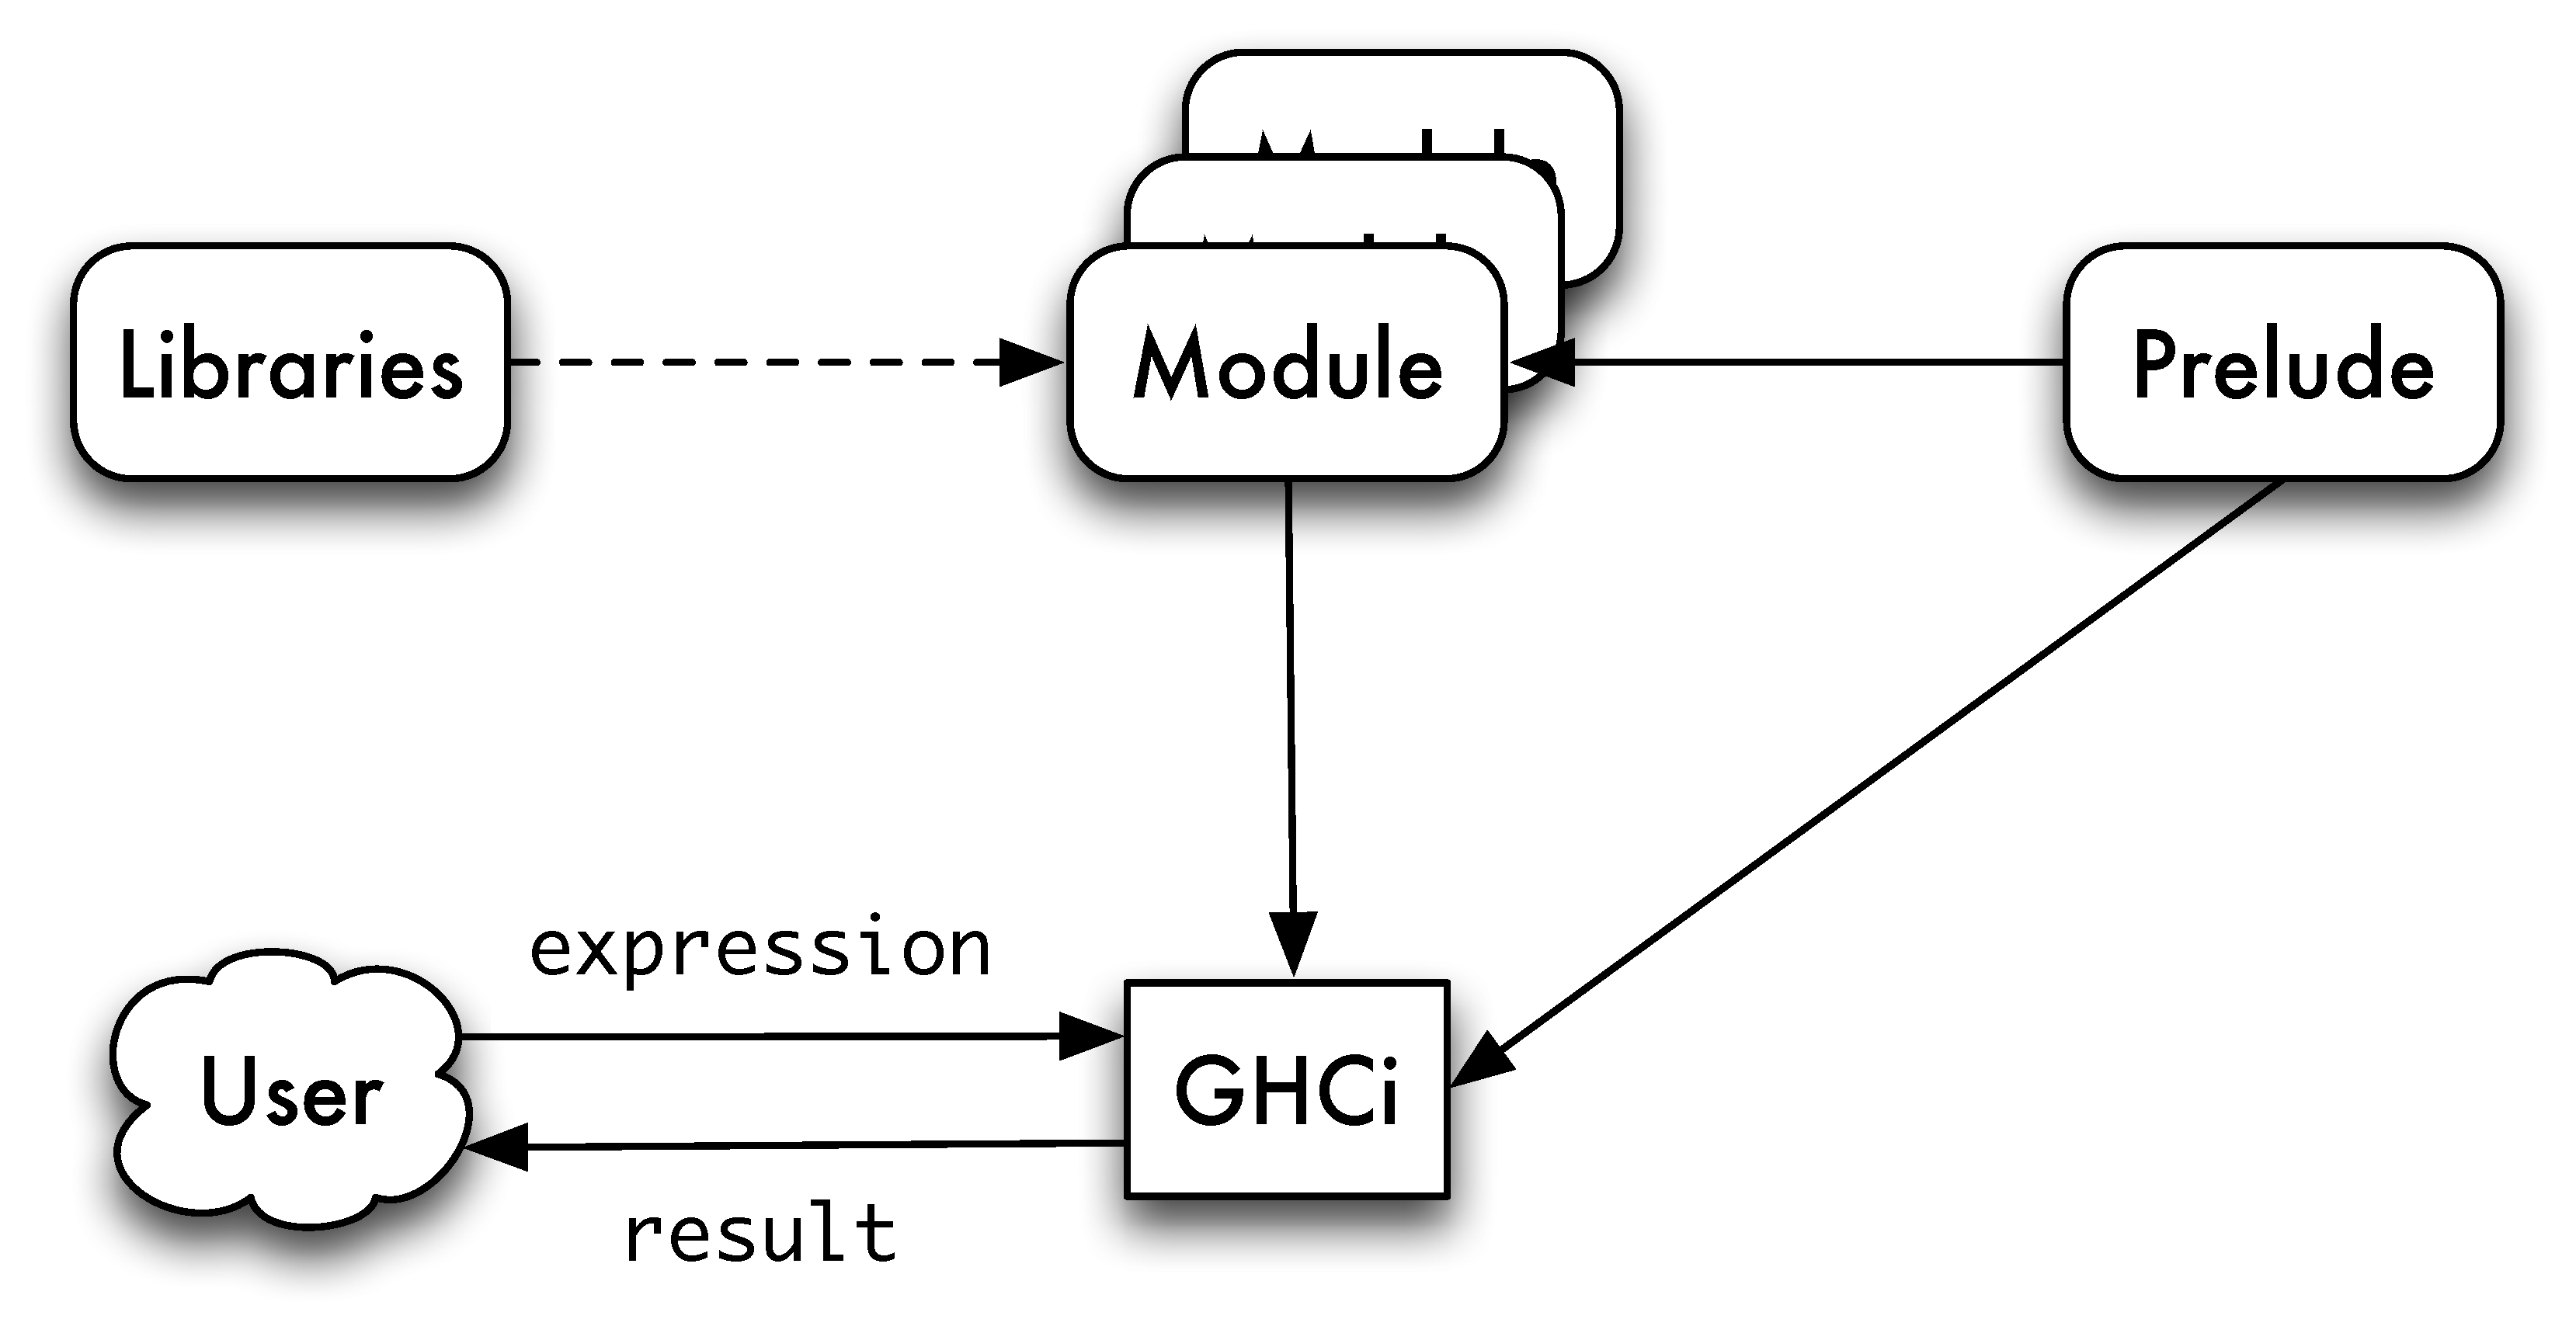
\includegraphics[width=4in]{Pictures/GHCiLibPrel.pdf}
\end{center} \index{GHCi!modules in}
\caption{GHCi, the Prelude and other modules}
\label{GHCiPreludeModules}
\end{figure}
 
A typical piece of computer software will contain thousands of lines of
program text. To make this manageable, we need to split it into smaller
components,  which we call modules. 

A \textbf{module}\index{modules} has a name
and will
contain a collection of Haskell definitions. To introduce a module called \texttt{Ant}
we begin the program text in the file thus:
\begin{alltt}\minx{Ant}\minx{module}
module Ant where
   ...
\end{alltt}
A module may also
\textbf{import}\minx{import} definitions from other modules. The module \texttt{Bee}
will import the definitions in \texttt{Ant} by including an \texttt{import} statement,
thus:
\begin{alltt}\minx{Bee}

module Bee where
import Ant
   ...
\end{alltt}
The import statement means that we can use all the definitions in
\texttt{Ant} when making definitions in \texttt{Bee}.
In dealing with modules in this text
we adopt
the conventions that
\begin{itemize}
\item there is exactly one module per file;
\item the file \texttt{Blah.hs} contains the module
\texttt{Blah}.
\end{itemize}
The module mechanism supports the libraries we discussed in
Section \ref{prelLibs}, but we can also use it to include code written by 
ourselves or someone else. 

The module mechanism allows us to control how definitions are imported
and also which definitions are made available or \textbf{exported}\minx{export} by a
module for use by other modules. We look at this in more depth in Chapter \ref{codes}, where we
also ask how modules are best used to support the design of software
systems.

In the light of what we have seen so far, Figure \ref{GHCiPreludeModules} illustrates a GHCi session.
like this: 
The current module will have access to the standard prelude, and to
those modules which it \texttt{imports}; these might include modules
from the standard libraries, which are found in the same directory as the
standard prelude\index{standard libraries!location of}. The user interacts with GHCi, providing
expressions to evaluate and other commands and receiving the results of
the evaluations.
\index{modules!introduction|)}

In the next section we look at how to work with multiple-module projects in GHCi, including the code for this text.

\section{Working with multiple-module projects}
\label{multipleModuleProgs}
\index{modules!multiple-module projects}

As we saw in the previous section, Haskell projects can be built from multiple modules, using the import and export mechanism. In this section we look at how projects can be downloaded and used; in particular how we can make sure that we're able to resolve all the dependencies of a particular project. We will see this in action with the Haskell package for this book, \texttt{Craft3e}.\index{Hackage!\texttt{Craft3e}}

Haskell projects, most of which consist of multiple modules, can be found on the Haskell Package Manager site, Hackage\index{Hackage}, and downloaded using Cabal\index{Cabal}. These projects themselves can depend on other packages, and this dependency and other \emph{project metadata} is contained in a \texttt{.cabal} file in the home directory of the package. The \texttt{.cabal} file summarises this information in a machine-readable format, allowing GHC to load all the dependencies of the project.

\subsection*{Working with \texttt{Craft3e}}

The code for this text is available on Hackage at 
\begin{center}
\url{https://hackage.haskell.org/package/Craft3e}
\end{center}
To download this to your machine type \texttt{cabal unpack Craft3e}. This will install the code for the book in a folder under \texttt{.cabal} in your home directory: the folder will be named \texttt{Craft3e-<version>}, where \texttt{<version>} is replaced by the current version number, \texttt{0.2.0.4} at the time of writing (2026-09-03).

Alternatively, if you are familiar with git and github, you can obtain the code from the github repository 
\begin{center}
\url{https://github.com/simonjohnthompson/haskellcraft}
\end{center}
by cloning the repository. As well as the code, this repository contains the source code for the book itself, and other miscellaneous material.

Whichever way you obtain the project, to work with the project, first change directory into the directory \texttt{Craft3e} (if you cloned the project from github) or \texttt{Craft3e-<version>} if you used \texttt{cabal unpack}. In either case you can then first run
\begin{alltt}
cabal build  
\end{alltt} 
which will install all the code that the book depends on; you just need to do this once, after obtaining the \texttt{Craft3e} project. Then to interact with the code in the project type
\begin{alltt}
cabal repl
\end{alltt}
This gives you a \texttt{ghci} prompt, but this time connected to GHC with all the dependencies available. You can work with ghci in the usual way.  The first time that you run \texttt{cabal repl} after obtaining the project may take time to complete, as the system installs dependencies: don't worry, this won't be a problem the next time you use it. 

Any new modules, such as \texttt{MyNewModule.hs} that you create \emph{within or below the Craft3e directory} will also have these dependencies available. These can be loaded with \texttt{:l MyNewModule}, and reloaded with \texttt{:r}, in the usual way.

If you choose to use an IDE such as VS Code you should open the Craft3e folder using the \textbf{Open Folder} command in the \textbf{File} menu. This will ensure that dependencies are visible, and the built-in terminal will be opened in the same directory. You can then use the Cabal commands just as they are described above.  VS Code is enhanced with HLS using the \texttt{haskell.haskell} extension, which is documented and downloadable from here:
\begin{center}
  \url{https://marketplace.visualstudio.com/items?itemName=haskell.haskell}
\end{center}
The next section revisits the picture example of Chapter
\ref{intro}, which is used to give a practical illustration of modules.


\begin{figure}[p]
\begin{alltt}\minx{Picture}
module Pictures where

type Picture = ....

-- The horse example used in Craft3e, and a white picture.

horse , white :: Picture
horse = ....
white = ....

-- Getting a picture onto the screen.

printPicture :: Picture -> IO ()
printPicture = ....

-- Reflection in vertical and horizontal mirrors.

flipV , flipH :: Picture -> Picture
flipV = map reverse
flipH = reverse

-- One picture above another. To maintain the rectangular 
-- property, the pictures need to have the same width.

above :: Picture -> Picture -> Picture
above = (++)

-- One picture next to another. To maintain the rectangular 
-- property, the pictures need to have the same height.

beside :: Picture -> Picture -> Picture
beside = zipWith (++)

-- Superimpose two pictures (assumed to be same size). 

superimpose :: Picture -> Picture -> Picture
superimpose = ....

-- Invert the black and white in the picture.

invertColour :: Picture -> Picture
invertColour = ....

\end{alltt}
\caption{A view of the \texttt{Pictures} module.}
\label{pictScript}
\vspace*{-12pt}
\end{figure}

\section{A second example: pictures}\label{picModuleEx}
\index{pictures}
\markright{A second example: \runinghead pictures}

The running example in Chapter \ref{intro} was of pictures, and we saw there that there are two implementations of these functions, one in \texttt{Pictures.hs} giving an `ASCII art' version, and the other in \texttt{PicturesSVG.hs} rendering pictures in a web browser.\minx{PicturesSVG}
\begin{itemize}\label{ShowBrowser}
\item
To use \texttt{PicturesSVG.hs}, open GHCi on this module like this:
\begin{alltt}\minx{ghci}
ghci PicturesSVG.hs
\end{alltt}
To show a picture in the browser, evaluate it using \texttt{render} as in \index{SVG!display in browser}
\begin{alltt}
render (horse `beside` (flipV horse))
\end{alltt}
This will give a browser display as shown in Figure \ref{svgpix}, page \pageref{svgpix}. The image in the browser will update automatically when you call \texttt{render} on another picture; if you would prefer to do this manually, use the file \texttt{showPic.html} instead.

\item
To use the `ASCII art' version, run
\begin{alltt}
ghci Pictures.hs
\end{alltt}
To show a picture in the terminal you need to use the function
\begin{alltt}\minx{printPicture}
printPicture :: Picture -> IO ()
\end{alltt}
which is used to display a \texttt{Picture} on the screen. The type
\texttt{IO} is a part of the Haskell mechanism for input/output
(I/O).\index{I/O}
We examine this mechanism in detail in Chapter \ref{io}; for
the present it is enough to know that if \texttt{horse} is the name of the
picture used in the earlier examples, then the effect of the function application
\texttt{\ printPicture horse\ } 
is the display
\begin{center}
{\footnotesize
\newlength{\blah}
\settowidth{\blah}{\texttt{............}}
\begin{minipage}{\blah}
\begin{alltt} 
.......##... 
.....##..#..
...##.....#.
..#.......#.
..#...#...#.
..#...###.#.
.#....#..##.
..#...#.....
...#...#....
....#..#....
.....#.#....
......##....
\end{alltt}
\end{minipage}
}
\end{center}
first seen in Chapter \ref{intro}. Any \texttt{Picture} can be printed
in a similar way. 
The \texttt{Pictures} module is shown in Figure \ref{pictScript}.
\end{itemize}
In the remainder of this section we present a series of practical
exercises designed to use either of the modules
\texttt{Pictures.hs} and \texttt{PicturesSVG.hs}.

\begin{exercises}

\item Define a module \texttt{UsePictures} which imports
\texttt{Pictures} (or \texttt{PicturesSVG}) and contains definitions of \texttt{blackHorse} and \texttt{rotateHorse} which can use the definitions
imported from the pictures module.

\medskip
\noindent
In the remaining questions you are expected to add other definitions to
your module \texttt{UsePictures}.

\item How could you make the picture
\begin{center}

\includegraphics[width=1in]{Pictures/twoByTwo.pdf}
\end{center}
Try to find two different ways of getting the result. It may help to work
with pieces of white and black paper.

Using your answer to the first part of this question, how would you
define a chess (or checkers) board, which is an $8\times8$ board of alternating squares? 

\item 
Three variants of the last picture which involve the `horse' pictures
are
\begin{center}

\includegraphics[width=4in]{Pictures/chessHorse.pdf}
\end{center}
How would you produce these three?

\item
Give another variant of the `horse' pictures in the previous question,
and show how it could be created. Note: a nice variant is 
\begin{center}
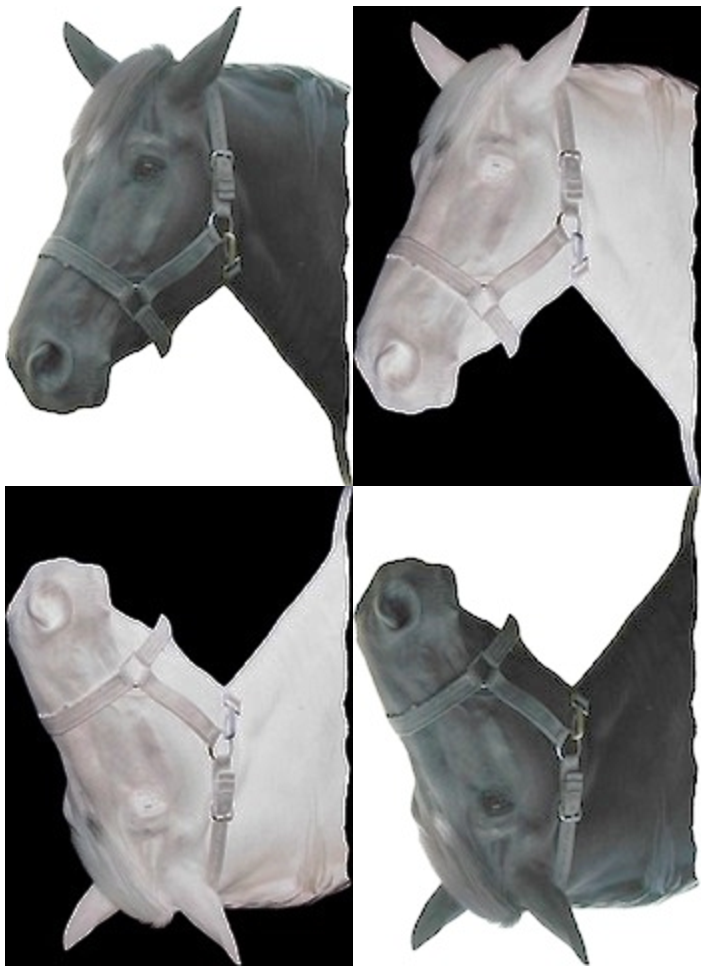
\includegraphics[width=1in]{Pictures/chessReflect.pdf}
\end{center}
\end{exercises}

\section{Errors and error messages}\label{errors}
\index{errors|(}

No system can guarantee that what you type is sensible, and GHCi is no
exception. If something is
wrong, either in an expression to be evaluated or in a script,
you will receive an \textbf{error message}\index{errors!error message}. Try typing
\begin{alltt}
2+(3+4
\end{alltt}
to the GHCi prompt. The error here is\index{errors!syntax}\index{syntax error}
in the \textbf{syntax}\index{syntax}, and is like a sentence in English
which does not have the correct grammatical structure, such as `Fishcake our
camel'. 

The expression
has too few parentheses: after the `\texttt{4}', a closing parenthesis is expected, to match with the
opening parenthesis before `\texttt{3}'. The error message says that something is wrong, but in fact it's not to do with indentation, but rather the lack of a closing parenthesis:
\begin{alltt}
<interactive>:1:7: error: [GHC-58481]
    parse error (possibly incorrect indentation or mismatched brackets)\end{alltt}
In a similar way typing \texttt{2+(3+4))} results in the message
\begin{alltt}
<interactive>:2:8: error: [GHC-58481] parse error on input ‘)’
\end{alltt}
which this time says that (one of) the closing parentheses causes a problem. Now try typing the following expression. 
\begin{alltt}
double square
\end{alltt}
This gives a \textbf{type} error, since \texttt{double} is applied to the
function \texttt{square}, rather than an integer:
\index{type error}\index{errors!type}
\begin{alltt}
<interactive>:5:1: error: [GHC-39999]
    • No instance for ‘Show (Integer -> Integer)’
        arising from a use of ‘print’
        (maybe you haven't applied a function to enough arguments?)
    • In a stmt of an interactive GHCi command: print it\end{alltt}
The message indicates that the system is trying to print something of type 
\texttt{Integer -> Integer}, that is a \emph{function} from integers to integers. It's a bit confused, but says that maybe a function has been applied to too few arguments. That's not the case here, but it might point us to the fact that there's an incorrect function application here: \texttt{double} has been applied to a function rather than a number.


When you get an error message like the one above you need to look
at how the \textbf{term},
in this case \texttt{square} of type \texttt{Integer -> Integer}, does not match the
\textbf{context} in 
which it is used: the context is given in the second line (\texttt{double square})
and the type required by the context, \texttt{Integer}, is given in the last line.

Type errors do not always give rise to
such well-structured error messages. Typing
either \texttt{4 double} or \texttt{4 5} will give rise to 
a message like

\begin{alltt}
<interactive>:6:1: error: [GHC-39999]
    • Could not deduce ‘Num a0’
      from the context: (Num a, Num ((a -> a) -> t))
        bound by the inferred type for ‘it’:
                   forall {a} {t}. (Num a, Num ((a -> a) -> t)) => t
        at <interactive>:6:1-8
      The type variable ‘a0’ is ambiguous
      Potentially matching instances:
        instance Num Integer -- Defined in ‘GHC.Num’
        instance Num Double -- Defined in ‘GHC.Float’
        ...plus three others
        ...plus one instance involving out-of-scope types
        (use -fprint-potential-instances to see them all)
    • In the ambiguity check for the inferred type for ‘it’
      To defer the ambiguity check to use sites, enable AllowAmbiguousTypes
      When checking the inferred type
        it :: forall {a} {t}. (Num a, Num ((a -> a) -> t)) => t
\end{alltt}
We will explore the technical details behind these messages in a later
chapter; for now it is sufficient to read these as `Type Error!'. One thing we can focus on, though, is the place that it says the error occurs: suppose that this was inside a larger program, it would still indicate the appearance of \texttt{4 double} as giving rise to the problem. So, \emph{always take note of where an error is said to occur.}

The last kind of error we will see are \textbf{program errors}. Try the
expression
\index{errors!program}\index{program error}

\begin{alltt} 
4 `div` (3*2-6)
\end{alltt}
We cannot divide by zero (what would the result be?) and so we get the message

\begin{alltt}
*** Exception: divide by zero
\end{alltt}
indicating that a division of \texttt{4} by \texttt{0} has occurred.
More details about the error messages produced by GHCi
can
be found in Appendix \ref{hugsErrors}.
\index{errors|)}



\begin{summary}
The main aim of this chapter is practical, to acquaint the reader with the 
GHCi implementation of Haskell. We have seen how to write simple Haskell
programs, to load them into GHCi and then to evaluate expressions which use
the definitions in the module.

Larger Haskell programs are structured into modules, which can be
imported into other modules. Modules support the Haskell library
mechanism and we illustrate modules in the case study of \texttt{Pictures}
introduced in Chapter \ref{intro}.

We concluded the chapter with an overview of the possible syntax, type 
and program errors in expressions or scripts submitted to GHCi. 

The first two chapters have laid down the theoretical and practical
foundations for the rest of the book, which explores the many aspects of
functional programming using Haskell and GHCi.
\end{summary}
%\end{document} 


